\documentclass[12pt]{template}
\usepackage{fancyhdr}
\usepackage{caption}
\begin{document}
\section{使用事件描述预测事件参与人数}
\subsection{概述}
上一章证明了事件描述对事件参与人数有显著的影响,因此,通过事件描述来预测参与人数便是顺理成章的了。 所以,接下来本章会提出三种预测器来预测二者之间的关系。这三种预测器分别是线性回归,带卷积层的神经网络和带GRU的神经网络。接下来,本章将分别对这三个预测器进行详细的描述。

\subsection{线性回归预测器}
线性回归是最简单的一种回归方法,同时只要二者关系是正相关的,在大多数情况下线性回归也有着不错的效果,所以这里也是把线性回归作为选择之一的原因。同时,线性回归也是本次实验的基线。在实验中,我们并没有采用最传统的线性回归,而是采用了拉索回归。原因是上一章我们假设事件描述对事件参与人数的影响主要由描述中的某些词导致的。所以这里在损失函数中加入L1正则来突出某些词的作用。此预测器及其损失函数如下:
% lasso function
\[argmin\left\{\frac{1}{N}\displaystyle\sum_{i=1}^{N}(y_i-\beta_0-\displaystyle\sum_{j}\beta_jx_{ij})^2\right\}
    \]
\[subject\ to \quad \displaystyle\sum_{i}|\beta_i|<\alpha
    \]
\[loss\ function: MSE+\sigma*\sum|\beta|
\]

在实现中,为了与后面两个分类器统一,我们使用了输出维数为1的单层线性神经网络,并采用了\textit{l1}正则。预测器的输入是序列化后的文本,目标(\textit{target})及输出则是参与人数。

\subsection{带卷积层的神经网络}
在使用线性回归做预测器时,我们假设各属性对结果的影响是互相独立,不受出现顺序影响的,即\(d(w|s_0)=d(w|s_0')=d(w)\),其中\textit{w}为词,\(s_0,s_0'\)为不同排列的相同的文本序列,\textit{d}为某个不存在的影响函数。但显然这个假设在现实中是不成立的,在自然语言中,词的出现顺序是非常重要的信息。例如在一段事件描述中,\textit{we will hold the meeting in a church}与\textit{church a in meeting the hold will we}这两句话在线性规划的眼中是没有区别的,但显然以人的眼光看,第二句话是没有意义的。因此,为了将文本的序列信息纳入考量范围,这里我们采用了带卷积的神经网络,如图\ref{f21}
\begin{figure}[htbp]
    \centering
    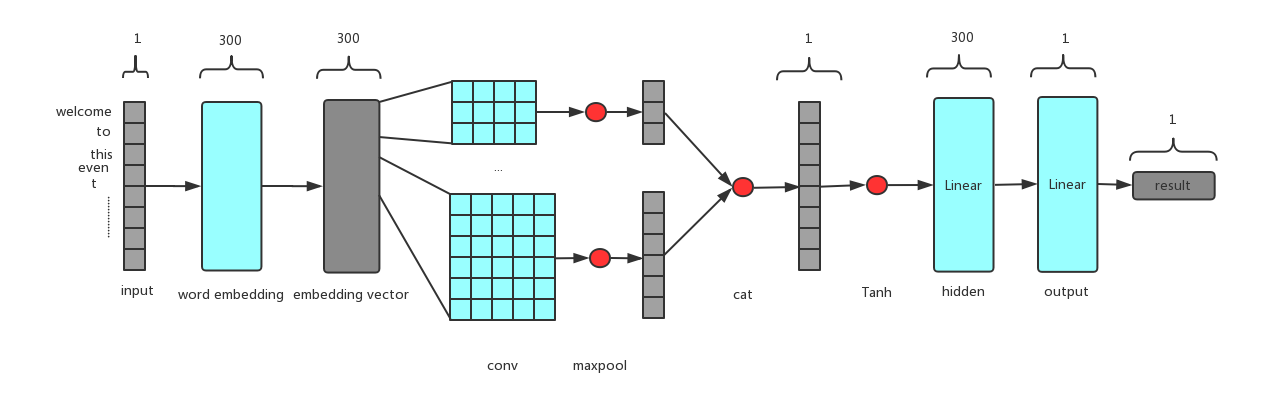
\includegraphics[width=16cm]{conv_ranker.png}
    \caption{带卷积层的神经网络}
    \captionsetup{font=small,margin=30pt}\caption*{图中灰色的方块表示向量,蓝色的表示网络,红色的圆点表示算符。在计算过程中,输入是文本序列,然后首先经过词向量层转换成词向量,然后进行卷积和池化(\textit{max-pooling}),将结果拼接起来,然后使用双曲正切(\textit{tanh})归一话,最后经过一个带隐含层的线性前馈神经网络输出最终结果。}
    \label{f21}
\end{figure}
\end{document} 